\section{Uppgift 7}\label{uppgift-7}

\subsection{Instruktioner}
\begin{verbatim}
7. Skriv ett program som låter användaren mata in värden till de tre
   heltalsvariablerna var1, var2 och var3. Programmet skall sedan för varje
   påstående a) – e) lagra värdet av påståendet i den booleska variabeln svar
   och därefter skriva ut värdet av svar , försett med lämplig ledtext:

    a) Talet var1 är jämnt delbart med 7.
    b) Talet var3 är inte jämnt delbart med talet var2.
    c) Talet var1 är större än minst något av talen var2 och var3.
    d) Talet var1 är större än talet var2, som i sin tur är större än talet var3.
    e) Talet var1 är större än ett av talen var2 och var3, men inte större än båda.

   Tips: För att kolla om något tal är jämnt delbart med ett annat,
         använd modulus-operatorn %!
\end{verbatim}


\subsection{Lösning}
\subsubsection{Funktion}
% TODO: Funktion på %7.
\subsubsection{Kommentar}
% TODO: Kommentar på %7.

\subsubsection{Källkod}\label{uppgift-7_src}
%\begin{listing}[H]
    \inputminted[linenos]{java}{src/Lab1Uppg07.java}
    \caption{Lab1Uppg07.java}
    \label{Uppg7src}
%\end{listing}

\subsubsection{Skärmdump}
\begin{figure}[htbp]
    \centering
        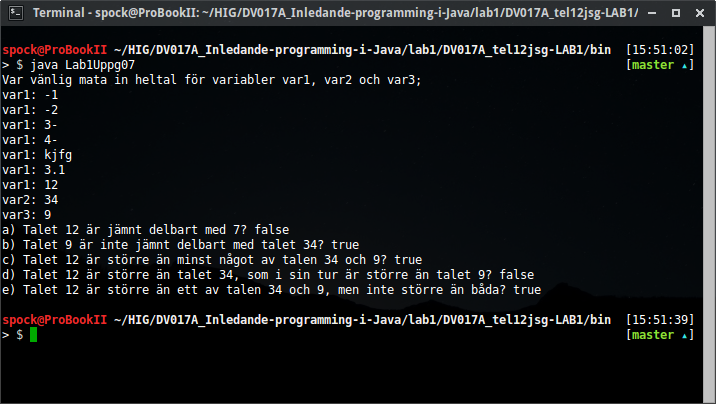
\includegraphics[width=\linewidth]{img/07.png}
    \caption{Körning av koden till Uppgift \ref{uppgift-7}}
    \label{fig:screenshot-07}
\end{figure}
